The physical scattering process producing speckle in the cone is perhaps best
understood in context of the simplified model shown in
\Figure{fig:plasmongeosimple}.  The model is general, but for the sake of
discussion it is assumed to be the planar scattering structure for SPP
excitation in the setup described in \Chapter{ch:experimental} (see
\Figure{fig:experimentalsetup}).  

The process is thought of as follows: SPPs are excited and come into existence
within the elliptical region of an evanescent wave created by the incident
beam (in the $x$-$z$ plane).  The SPP then propagates, potentially out of the
elliptical region, until either decaying as heat or re-radiated as a photon
out into the cone.  The maximum propagation distance is given as per
\Section{sec:sppphysicalchar}.  SPPs which decay as heat or otherwise do not
re-radiate as photons into the cone are unobservable in this experiment and
are therefore neglected.  During propagation, the SPP follows a scattering
path, accumulating phase by visiting one or more in-plane scatterers.  The
final scatterer is the location where SPPs scatter out of plane into the cone.
The superposition of light with phases set by all SPPs paths is responsible
for the observed speckle in the cone.

Restated, the individual components of the scattering model shown in
\Figure{fig:plasmongeosimple} are:
\begin{itemize}
\item An elliptical \textit{illuminated region}, representing the incident
				evanescent field used to excite SPPs.
\item \textit{Scatterers}, fixed point defects, assumed to be randomly
				distributed, which modify the in-plane momentum of an SPP and
				optionally cause its re-radiation as a photon out of plane into the cone. 
\item A \textit{scattering path}, the ordered sequence of
				scatterers an SPP visits before exiting the system.  
\item An SPP \textit{creation point}, where an SPP comes into existence and
				begins accumulating phase.
\end{itemize}
\begin{figure}[ht]
\centering
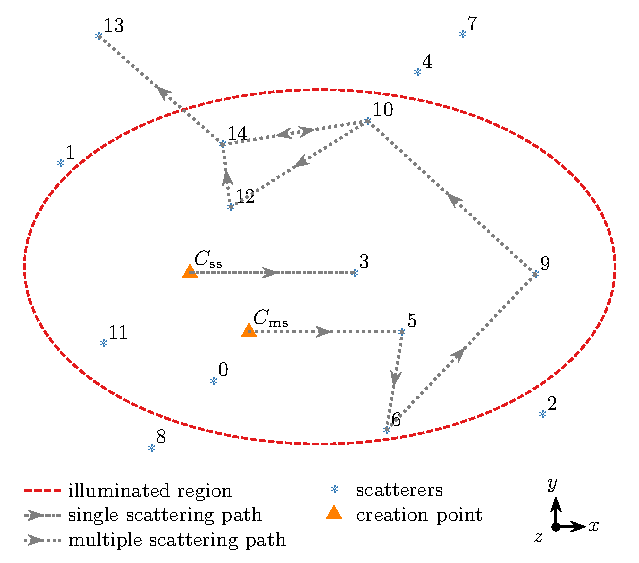
\includegraphics[keepaspectratio]{scatteringmicro/figures/montecarlogeosimple.pdf}

\caption{A simplified SPP scattering model.  An SPP is excited within the
				illuminated region at its creation point and follows a scattering path
				amongst fixed point scatterers (numbered).  The scattering path can
				include one (single scattering) or more (multiple scattering)
				scatterers.  The beam creating the illuminated region is incident from
				the ${+}x$ direction.}

\label{fig:plasmongeosimple}
\end{figure}

Physically there are two possible in-plane scattering processes, both of which
are depicted in \Figure{fig:plasmongeosimple}.  The first is \textit{single
scattering}, whereby only one scatterer is visited in each path from source to
observation.  An example single scattering path is given in
\Figure{fig:plasmongeosimple} by the path $\{C_\mathrm{ss},3\}$, where an SPP
is created at $C_\mathrm{ss}$, propagates to scatterer $3$, then is
re-radiated into the cone.

In addition to single scattering, there exists a much more interesting and
phenomenologically complex process known as \textit{multiple scattering}.  In
multiple scattering, each path from source to observation contains multiple
scattering events.  An example multiple scattering path is shown
in \Figure{fig:plasmongeosimple} by the path
$\{C_\mathrm{ms},5,6,9,10,12,14,10,14,13\}$.  This path serves to illustrate
several important assumptions which are made regarding the behavior of a multiple scattering
path:
\begin{itemize}
\item The scatterers are randomly distributed (true for single
				scattering as well).
\item The same scatterer has the possibility of being visited an arbitrary
				number of times, e.g.\ $\{10,12,14,10,14\}$.
\item Closed loop and time reversed paths are possible, e.g.\ $\{10,12,14\}$.
				In these cases the accumulated phase is the same regardless of
				direction, e.g. $\{10,12,14\} \equiv \{14,12,10\}$.  Such paths are
				said to have \textit{time reversal symmetry}.
\end{itemize}

Note the first scatterer visited in both example paths for single and multiple
scattering, $3$ and $5$ respectively, are directly downstream of their SPP
creation points.  That is to say, to a good approximation, the first scatterer
is always located in the ${+}x$ direction; in the coordinate system of
\Figure{fig:plasmongeosimple}, an SPP at its creation point has momentum in
the ${+}x$ direction.  Including this assumption in the scattering model
implies not all scatterers can be reached in a single scattering process or as
the first scatterer of a multiple scattering process (e.g.\ scatterers
1, 13, 8, 4, and 7).

\subsection{Phase Accumulation and Extension to the Far Field} 
The local in-plane scattering process in the simplified model of
\Figure{fig:plasmongeosimple} will now be extended to describe light in the
cone.  Assume that each scatterer has a location given
by the Cartesian coordinates $(x,y,z=0)$, where the central point of the
prism's hypotenuse on the far surface of the film is the origin
$(0,0,0)$.  The central point of the focus of the incident Gaussian 
beam (the illuminated region) is also coincident at $(0,0,0)$.

In the cone, the detector (a two-dimensional image sensor) is assigned the
coordinates $(x^\prime,y^\prime,z^\prime)$.  Again, the film is in the
$x$-$y$ plane and the incident light in the $x$-$z$ plane.
The field on the detector has either two or three phase contributions,
depending on the scattering order. The first, $\varphi_\mathrm{loc}$, comes
from the phase of the local SPP field propagating on the surface in the
${+}x$ direction to the first scatterer,
\begin{equation}
\varphi_\mathrm{loc} = \ksp x.
\label{eqn:smicrofirstphase}
\end{equation}
In the example paths of \Figure{fig:plasmongeosimple}, the variable $x$ in
\Equation{eqn:smicrofirstphase} would be the $x$
coordinate of either scatterer $3$ or $5$.  Given an SPP is in phase with the
exciting field, the choice of the origin and this first phase is arbitrary,
but is expressed as in \Equation{eqn:smicrofirstphase} for simplicity.

The second phase contribution is $\varphi_\mathrm{ff}$: the phase accumulated
from the final out of plane scatterer to the detector in the far field,
\begin{equation}
\varphi_\mathrm{ff} =
k_0\sqrt{{(x-x^\prime)}^2+{(y-y^\prime)}^2+{(z-z^\prime)}^2},
\label{eqn:smicrosecondphase}
\end{equation}
where $x$, $y$, and $z$ in \Equation{eqn:smicrosecondphase} would assume the coordinates of the final scatterer
($3$ or $13$ in the example paths of \Figure{fig:plasmongeosimple}).

Following Equations~\ref{eqn:smicrofirstphase} and~\ref{eqn:smicrosecondphase},
the field on the detector for the $n$th path in the case of single scattering is given by
\begin{align}
\mathbf{E}_n(x^\prime,y^\prime,z^\prime) &=
\mathbf{E}_n\exp\bigl(\mi(\varphi_\mathrm{loc}+\varphi_\mathrm{ff})\bigr)\\
&= \mathbf{E}_n\exp\!\left(\mi\ksp x + %
\mi k_0\sqrt{{(x-x^\prime)}^2+{(y-y^\prime)}^2+{(z-z^\prime)}^2}\right).
\label{eqn:smicrosinglescattering}
\end{align}
Or in spherical coordinates, with the detector at
$(\rho^\prime,\theta^\prime,\phi^\prime)$,
\begin{align}
				\mathbf{E}_n(\rho^\prime,\theta^\prime,\phi^\prime) &= \mathbf{E}_n\exp\Bigl(\mi\ksp x \\
&+ \mi k_0\sqrt{{(\rho^\prime\sin\theta^\prime\cos\phi^\prime
x+x)}^2+{(\rho^\prime\sin\theta^\prime\sin\phi^\prime+y)}^2+{(\rho^\prime\cos\theta^\prime+z)}^2
} \Bigr).
\label{eqn:scattspherical}
\end{align}
Again, $x$, $y$, and $z$ are the coordinates of the sole scatterer in an
individual path of the single scattering process.  Note that the
refractive index change from prism to air has been neglected.  To a good
approximation, the hemispherical geometry imparts only a constant phase to the
each scattering path, and therefore has no effect on the speckle pattern.

For a system with $M$ total scatterers and $N \leq M$ scatterers downstream of
a creation point within the illuminated region, a single scattering process
will produce $N$ unique phasors over $N$ paths.  The $n$th path has a
phase $\varphi_n$ given by the sum of the local and far field phases,
\begin{equation}
\varphi_n = \varphi_\mathrm{n,loc}+\varphi_\mathrm{n,ff}. 
\end{equation}

Assuming each of the $N$ scatterers is visited with equal probability and SPPs
re-radiating as photons are scattered isotropically into the cone, the field
on the detector is given by the coherent superposition of the paths,
\begin{align}
\mathbf{E}(x^\prime,y^\prime,z^\prime) &=
\sum_{n=0}^{N-1}
\mathbf{E}_n \me^{\mi{(\varphi_\mathrm{n,loc}+\varphi_\mathrm{n,ff})}}\\
&=
\sum_{n=0}^{N-1}
\mathbf{E}_n \me^{\mi{\varphi_\mathrm{n}}},
\end{align}
where $\mathbf{E}_n$ is the fractional contribution of each scattering path to
the total amplitude of the electric field $\mathbf{E}_0$ set by the incident
beam, such that
\begin{equation}
\sum_{n=0}^{N-1}\mathbf{E}_n = \mathbf{E}_0.
\end{equation}

For a multiple scattering process, a third phase term,
$\varphi_\mathrm{ms,n}$, must be included for each scattering path.
$\varphi_\mathrm{ms,n}$ accounts for in-plane multiple scattering, where each
of $N$ total paths visits $K$ scatterers amongst the $M$ total.  If the
ordered scattering sequence for the $n$th path is given by $\{S_{n,0} \ldots
S_{n,{K-1}}\}$, and the positions of the $k$th scatterer in the path sequence
is $(x_{S_{n,k}},y_{S_{n,k}},z=0)$, the phase accumulated for the $n$th path from
multiple scattering is
\begin{equation}
\varphi_\mathrm{ms,n}=\sum_{k=0}^{K-2}
\ksp \sqrt{{(x_{S_{n,{k+1}}}-x_{S_{n,k}})}^2+{(y_{S_{n,{k+1}}}-y_{S_{n,k}})}^2}.
\label{eqn:multiplescatteringphase}
\end{equation}
The length of $S_n$ and its ordered sequence is assumed to be produced by a stochastic
process and will vary from path to path.  The field on the detector
for multiple scattering is then given by the superposition of all paths from
creation to detector
\begin{equation}
\mathbf{E}(x^\prime,y^\prime,z^\prime) =
\lim_{N\to\infty}
\sum_{n=0}^{N-1}
\mathbf{E}_n
\exp\!\big({\mi{(\varphi_\mathrm{n,loc}+\varphi_\mathrm{n,ff}+\varphi_\mathrm{n,ms})}}\big).
\label{eqn:smicromsphase}
\end{equation}

\Equation{eqn:smicromsphase} is akin to the path integral formulation of
quantum mechanics.  By letting $N\to\infty$, all possible sequences of $S_n$
(again, produced by a yet unspecified stochastic process) will be explored by
the multiple scattering paths weighted by $\mathbf{E}_n$.  In the present set
of experiments with a \SI{50}{\milli\watt} diode laser, the limit in
\Equation{eqn:smicromsphase} is for all practical purposes fulfilled.
Furthermore it will be assumed that the number of scatterers $M$ is sufficient
to produce speckle with statistics given by the random phasor sum model
(\Equation{eqn:phasorsum}).

%\Equation{eqn:smicromsphase} also captures single scattering if $k=1$.

%can be expressed differently to account
%for both single and multiple scattering.

\subsection{Transition from Single to Multiple Scattering}
The transition from the single to the multiple scattering occurs roughly upon
fulfillment of the Ioffe-Regel criterion~\cite{ioffe1960non}, when the
transport mean free path $l^*$ is much larger than the spatial frequency of
the optical wave, or
\begin{equation}
k l^* \approx 1
\end{equation}
where $k=\omega/c$ as usual.  The transport mean path is defined as the
characteristic distance over which the incident wave is scattered out of its
incoming direction~\cite{berkovits1994correlations}.  This is the optical
analog of electron transport in condensed matter physics.  There, one would
use the Fermi wavenumber $k_F$ and take $l^*$ to be the mean free path.
Materials for which $k_F l^* \gg 1$ are conductors, and materials for which
$k_F l^* \ll 1$ are insulators.  The multiple scattering regime can also be
defined in terms of the sample length $L$, such that if $l^* \ll L$ and $1/(k
l^*) \ll 1$, the system can be thought to be the multiple scattering regime.

\subsection{Sensitivity and Scattering Paths}
\label{sec:senspaths}
The number of scatterers visited in the sequence $S_n$ of a scattering path is
fundamental in capturing the essence of both single and multiple scattering.
Consider a random phasor sum consisting of $N$ phasors.  In the case of single
scattering, the $N$ phasors map directly to $N$ scatterers, and the problem is
equivalent to a random walk in $\mathbb{R}^2$.  Assuming all scattering paths
equally probable, all phasors will have equal magnitude.  Furthermore, the
phasor magnitude is assumed to be unity, whereby the mean value of the phasor
sum is $\sqrt{N}$.  Upon the addition of an additional ($N+1$) scatterer, the
magnitude of the phasor sum for single scattering is therefore altered by an
(ensemble averaged) value of $1/N$.

Determining the sensitivity of a speckle pattern to the addition of a single
scatterer in the multiple scattering regime is much more complicated; the
mathematics of which are beyond the scope of the present investigation.  Using
a ladder-operator approach similar to that of \name{Feng}, \name{Lee},
\name{Stone}, and \name{Douglas}~\cite{feng1986sensitivity},
\name{Berkovitz}~\cite{berkovits1991sensitivity} gives an ensemble averaged
sensitivity of $1/N^3$ for multiple scattering in the two-dimensional slab
geometry~\cite{nieuwenhuizen1993role}.

%Xxxxxxxxxx is the cone really isotropic?  show a picture xxxxxxxxxxx
